\documentclass[11pt,oneside,twocolumn,a4paper]{article}

\usepackage{graphicx}
\usepackage[footnotesize,bf]{caption}
\usepackage{fancyhdr}
\usepackage[numbers,sort&compress]{natbib}
\usepackage[usenames,dvipsnames]{color}
\usepackage{enumitem}
\usepackage[colorlinks=true, linkcolor=BrickRed, citecolor=Blue, urlcolor=Blue, filecolor=Blue]{hyperref}
\input{jdefs.tex}

\addtolength{\topmargin}{-0.8in}
\addtolength{\textheight}{2.0in}
\addtolength{\textwidth}{0.95in}
\addtolength{\oddsidemargin}{-0.45in}

\fancyhead[LE,RO]{\thepage}
\fancyhead[LO,RE]{Pat Scott}
\fancyhead[C]{STFC ERF Case for Support: The astroparticle road to new physics}
\fancyfoot[C]{}
\renewcommand{\headrulewidth}{0.4pt}
\renewcommand{\footrulewidth}{0pt}
\pagestyle{fancy}

\author{Pat Scott}
\date{}

\setlist{nolistsep}

\begin{document}

\thispagestyle{fancy}

\subsubsection*{Research track record and career vision}

My overarching goal is to perform cutting-edge astroparticle research: to discover and characterise new physics and symmetries of nature, and their impacts upon astronomical observations. I ultimately plan to build and lead a large, strong and dedicated research group centred on the interface of particle physics and astronomy. This group will focus on dark matter (DM) and physics beyond the Standard Model (SM) of particle physics, with particular emphasis on quantitative, multi-messenger assessments of the leading theories of the day for new physics.  The ERF will give me the opportunity to build this group, providing the stability to apply for further external funding to hire postdocs of my own, and take on students. This will allow me to take my leadership in astroparticle physics to the next level, and eventually run such a group in earnest as permanent faculty.

I have just over 2 years postdoctoral experience, 22 published or submitted articles in refereed journals, 10 refereed proceedings and 1239 citations.  My work includes some of the most rigorous global fits for new particle theories to date with data from indirect dark matter searches [1,6,12 in publication list].  This work significantly improved constraints on supersymmetric dark matter, and was only possible through dedicated collaborations between myself and the relevant experiments: first with gamma-ray data from the \emph{Fermi} Large Area Telescope (LAT) [12] and the High Energy Stereoscopic System (HESS) [6], then with IceCube neutrino events [1].  I also played a pivotal role in the recent correction of the chemical composition of the Sun [13], which impacts many areas of astronomy and astroparticle physics.

I have won multiple externally-funded research grants and fellowships: The Banting Fellowship from the Canadian Government (Canada's most sought-after postdoctoral fellowship), the CfA Fellowship from Harvard University (which I declined), two other major grants and 7 smaller competitive travel fellowships. I won The Arrhenius Prize at Stockholm University for my PhD research (in particular my global fit work), the Bok Prize from the Astronomical Society of Australia for the best Honours/Master thesis in astrophysics, and two University Medals for my Honours research at the Australian National University.

I have given 66 talks (19 invited) at international conferences and institutions, and chaired 5 sessions. I convened the Particle Astrophysics and Cosmology Track at the 2012 International Conference on High Energy Physics (ICHEP), organised 2 smaller conferences, and founded the McGill Astroparticle Seminar Series. I am an associate member of the IceCube Collaboration and an affiliated scientist of the \emph{Fermi}-LAT. I collaborate with leading astronomical and particle phenomenology groups all over the world: in the US, Canada, UK, Australia, NZ, Scandinavia and Germany.  I have refereed for 6 top-tier journals and authored 4 public astroparticle software packages. I created and lectured an official McGill course in numerical methods, have mentored 4 PhD and 5 Masters students, and am just about to serve on an external PhD defence committee for a student in Lisbon.

\subsubsection*{Scientific vision}

The identity of dark matter and the nature of physics at the TeV energy scale are two of the most pressing and fundamental questions in modern physics.  DM constitutes 80\% of the matter in the Universe and was discovered 80 years ago, but its composition remains a mystery.  With the activation of the Large Hadron Collider (LHC), discovery of the Higgs boson and construction of high-energy astrophysics experiments like the \emph{Fermi}-LAT, HESS-II, IceCube and SuperCDMS, we now stand on the doorstep of the TeV scale.  

Excitingly, many popular DM candidates are intrinsically linked to the appearance at the TeV scale of new physics beyond the Standard Model (BSM).  A Higgs mass of 125\,GeV itself even compels us to move beyond the SM: theoretically, this value should be orders of magnitude higher if the impact of SM virtual particles is taken into account.  If no other particles exist, then the very vacuum of our Universe is also unstable, and might undergo a catastrophic energy transition at any moment.  We also know that the SM is incomplete because it does not explain the excess of matter over antimatter in our Universe, nor that fact that neutrinos are massive.

Many different probes are sensitive to BSM physics: direct and indirect searches for DM, accelerator searches, and neutrino experiments.  Experiments such as CRESST, \emph{Fermi}-LAT and PAMELA may even already show tantalising hints of DM.  To make robust conclusions about the overall level of support for different BSM scenarios from such varied sources, a simultaneous statistical fit of all the data, fully taking into account all relevant uncertainties, assumptions and correlations is an absolute necessity.  This `global fit' approach is what I propose here.  Such holistic analyses exploit the synergy between different experimental approaches to its maximum potential, squeezing every last statistical drop of information possible from each source.  Robust analysis of correlated signals, in a range of complementary experiments, is \textit{essential} for claiming a credible discovery of DM or new physics at the TeV scale -- and indeed, even for definitively excluding theories.  This `win-win' situation is a particular feature of a global fit analysis, as even non-detections provide crucial physical insight into which theories and parameter regions are disfavoured.

This is an extremely demanding task, existing on the cusp of theory and experiment, astronomy and particle theory -- and requiring excellent understanding not only of the theories and experiments involved, but also many specialised statistical techniques and computer codes.  I am uniquely placed to lead this endeavour, with the extensive cross-disciplinary background in astrophysics and particle physics, theory and experiment, DM phenomenology, statistical and numerical methods required to make this ambitious proposal a reality.  Astroparticle experimental collaborations have so far carried out such global analyses only with my assistance: the examples to date have been my collaborations with the \emph{Fermi}-LAT [12 in publication list], HESS [6] and IceCube [1].

Whilst partial progress has recently been made (by various groups including myself, Roberto Trotta at Imperial, and our respective collaborators), the magnitude of the task and degree of technical difficulty have left global fits largely unexplored for the majority of theories and datasets.  With the startup of the LHC, vast amounts of additional data are rapidly becoming available at the TeV scale, making even analyses done in the past year obsolete.  \textit{Now} is precisely the time to invest in broadening the application and development of BSM global fits and their related computer codes, in order to deal together, in a consistent and holistic way, with a greatly expanded number of theories and the impending flood of new datasets.

\subsubsection*{Scientific Objectives}
\begin{enumerate}
\setlength{\itemsep}{2pt}
\item Identify the correct theory behind dark matter and TeV-scale BSM physics
\item Exclude large classes of other viable and popular dark matter and TeV-scale BSM theories
\item Distinguish between areas of parameter space giving rise to distinct astroparticle phenomena within single BSM theories
\end{enumerate}

\begin{figure}[t!]
  \centering
  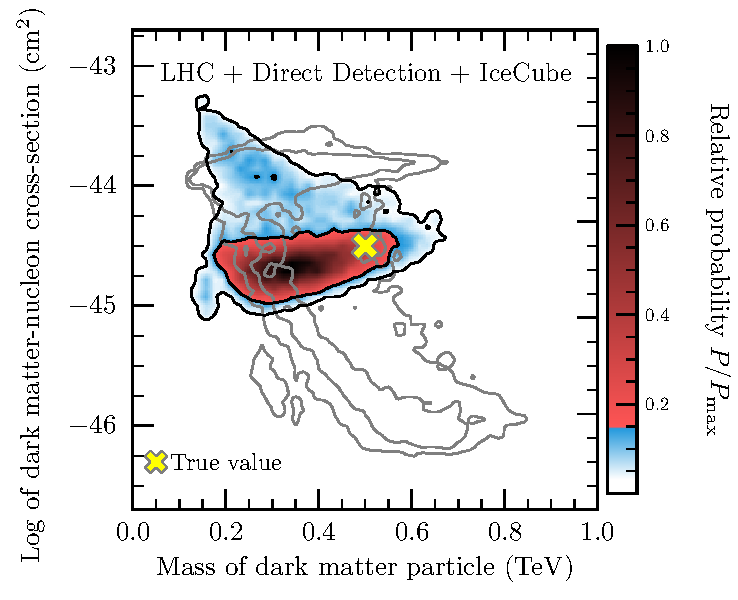
\includegraphics[width=0.93\linewidth]{URF_Proposal_Fig_1}
  \caption{An example global fit exploiting the synergy between experiments in the search for BSM physics and DM.  Grey contours show the result when LHC and XENON-100 direct detection data are used to constrain supersymmetry, in terms of the mass of the DM and its scattering cross-section with nucleons.  Shading shows how the picture changes when a mock detection of DM by the IceCube Neutrino Telescope is considered, corresponding to a specific point in the parameter space.  Shading gives the relative probability of the different parts of the parameter space, and contours give $1\sigma$ and $2\sigma$ regions.  The fit with IceCube data zooms in markedly on the true point, determining the scattering cross-section with about a factor of 100 better accuracy than without IceCube (at 68\% confidence level).  Based on [1] in publication list.}
  \vspace{-6mm}
  \label{example}
\end{figure}

\subsubsection*{Research Framework/Methodology}

An example of the utility of a global fit is shown in Fig.~\ref{example}.  Here probability distributions for the mass of supersymmetric DM, and its scattering cross-section with nucleons, are shown for two parameter scans.  In one scan (grey), LHC and direct detection data are used to constrain an example supersymmetric theory.  Two main regions of high probability exist: a horizontal region with large cross-sections, where the DM also has a large annihilation cross-section and its cosmological density it determined by DM-DM annihilation, and an almost vertical region extending to lower cross-sections, where the DM has a much lower annihilation cross-section and its cosmological density is determined mostly by co-annihilation of DM particles with other supersymmetric particles.  With LHC and direct detection data alone, there is no way to determine which of these regions is favoured, and therefore what physical process is primarily responsible for determining the amount of DM in the Universe.  When data from a future hypothetical detection of DM with the IceCube Neutrino Telescope are added (colour), the degeneracy is lifted, and the parameter space is constrained with high accuracy (a factor of 100 improvement in the cross-section).

The core statistical methodology is that of a composite likelihood-based global fit.  One first chooses a BSM physics scenario with some model parameters, and then calculates predicted experimental signatures of the model for arbitrary parameter combinations (gamma-ray fluxes, LHC event rates, etc).  Predictions are compared to experimental measurements, and a series of likelihood functions produced.  Such analyses have the added advantage of being able to fully deal with uncertainties in modelling assumptions or standard input data, by including them as additional parameters in the fit.  The entire exercise can be repeated for different BSM scenarios with different parameterisations, and the results compared to determine if the data strongly favour one scenario over another.

\subsubsection*{Core Research Fronts}

\textbf{Particle and astroparticle datasets:}
With Roberto Trotta and accelerator, direct detection and cosmic microwave background (CMB) experts at Imperial, I will include many new and updated observables in my global fits.  BSM searches with CMS and ATLAS at the LHC are essential inclusions, but notoriously difficult in all but the simplest BSM theories.  In consultation with Tapper, Buchm\"uller and the Imperial CMS group, I plan to develop approximate but detailed LHC likelihood functions for use in global fits, initially based on the most constraining CMS searches for supersymmetry, including the `razor' and `MT2' analyses.  Direct searches for DM like XENON-100, ZEPLIN and LUX will also play a pivotal role.  In collaboration with Araujo and Sumner at Imperial and the rest of the ZEPLIN/LUX collaboration, I will include full event-level data and detailed background models in the direct detection likelihoods of my global fits.  With Jaffe I will include the impacts of DM annihilation on the CMB, as seen by Planck.

I will leverage my contacts in \textit{Fermi}, IceCube and AMS-02 to include searches for cosmic anti-deuterons from Galactic DM annihilation with AMS-02, searches for DM annihilation in the Sun by IceCube, and combined searches for gamma rays from DM annihilation in all Milky Way dwarf satellite galaxies by \textit{Fermi}.   Together with the developers of the \textsf{GALPROP} cosmic ray propagation code, Trotta and I will develop a global fit analysis of \textit{Fermi} data from the Galactic centre, utilising nested sampling, Bayesian object detection and detailed diffuse emission templates.

\textbf{Theories:}
I will investigate the current leading candidates for new physics: 7-, 13-, 19- and 25-parameter phenomenological versions of the minimal supersymmetric standard model (MSSM), specific supersymmetry-breaking schemes such as Planck-scale-mediated, gauge-mediated, anomaly-mediated and gaugino-mediated scenarios, and models of extra dimensions.  I will also derive global constraints on more effective DM models, including Effective WIMPs, Sommerfeld-enhanced models, Two Higgs Doublet Models, Asymmetric DM, Isospin-Violating DM, Inelastic and Exciting DM.  This will allow me to test, refine and compare the viable regions of these models to a far greater extent than done previously.

\textbf{Statistical \& Numerical Methods:}
A core part of my ERF will be developing a second-generation BSM global-fitting software package, able to dynamically rewrite modules of its own code to implement new theories and adjust to new experimental datasets.  This will allow a degree of flexibility not before seen in statistical analyses of BSM theories, facilitating the analysis of vastly more theories and experimental signatures than has been done to date.  I intend to make this software, and its component physics codes, freely available to the community.

With the members of the new Imperial Centre for Inference and Cosmology (ICIC; Trotta, Jaffe, van Dyk et al), I will improve on the statistical and numerical aspects of global fit analyses.  I have particular expertise in optimisation/scanning algorithms, with extensive experience in both Bayesian and frequentist scanning methods (e.g. genetic algorithms, nested sampling).  I will leverage this expertise and the excellence of the ICIC to develop a new alternative scanning code for BSM searches, based on the strategy of differential evolution.

\textbf{Additional synergies} with my program exist within Imperial and the general London area.  Ellis, Fairbairn and colleagues in High Energy Theory at King's College might contribute to phenomenological aspects of the BSM fit program.  As I have shown previously, indirect DM detection also has cosmological implications, via consideration of ultracompact minihalos; my work in this direction would benefit from interaction with Jaffe and Contaldi (inflation and cosmological perturbations), and Rajantie (cosmic strings).

\subsubsection*{Timeline}

\noindent\textbf{Years 1--2} Develop:\\
$\phantom{xx}\bullet$ core second-generation global fitting code\\
$\phantom{xx}\bullet$ first LHC (few channels) likelihood module\\ 
$\phantom{xx}\bullet$ direct detection likelihood modules\\
$\phantom{xx}\bullet$ indirect detection likelihood modules\\
$\phantom{xx}\bullet$ differential evolution scanner\\
Publish:\\
$\phantom{xx}\bullet$ indirect detection likelihood code package paper\\
$\phantom{xx}\bullet$ direct detection likelihood code package paper\\
$\phantom{xx}\bullet$ differential evolution code paper\\
\noindent\textbf{Year 3}\\ 
$\phantom{xx}\bullet$ Publish phenomenological MSSM analyses\\
$\phantom{xx}\bullet$ first public release of code\\
\noindent\textbf{Year 4} Add/update observables:\\
$\phantom{xx}\bullet$ all LHC channels\\
$\phantom{xx}\bullet$ cosmic rays + propagation models\\
$\phantom{xx}\bullet$ gamma-rays\\
$\phantom{xx}\bullet$ neutrino telescope\\
$\phantom{xx}\bullet$ CMB limits on DM annihilation\\
Add theories:\\
$\phantom{xx}\bullet$ supersymmetry-breaking mediation models\\
$\phantom{xx}\bullet$ extra dimensions\\
$\phantom{xx}\bullet$ Two Higgs Doublet Models\\
$\phantom{xx}\bullet$ effective DM models\\
\noindent\textbf{Year 5} Complete and publish (for all theories):\\ 
$\phantom{xx}\bullet$ global parameter analyses\\
$\phantom{xx}\bullet$ extensive model comparison
\end{document}
